\chapter{Electronic Design}

At the core of any reliable system is a thoroughly planned electronics system. There are multiple aspects this subsystem must handle. Due to the rapidly increasing market and interest in multirotors there has been a wave of developers and designers creating devices for these specific purposes. The first and foremost is monitoring and controlling flight dynamics. This requires flight, speed and motor controllers.	

The on board computer will handle the data streams and control the non-real time peripherals. The device also needs to have networking capabilities to allow wireless communication during flights. For the drone to successfully navigate an environment it will need to better understand it's surroundings. To achieve successful navigation, a few onboard sensors have been looked at. Another useful and necessary function, will be the ability to illuminate a dark area. This will allow surveillance and condition monitoring of these unlit zones. Another design consideration is the provision for a sensor pack. This section of the study involves looking at potential external sensors and providing accessibility for them.

No system can operate without a sufficient power source. In the case of any robotic system it is important that every aspect of the design is optimised. To assist with that an electrical analysis is done to help pinpoint some of the major power consuming components. This analysis will also help to evaluate the required power source. The capacity of the power supply is limited by weight and should be optimised to the lifting capacity of the platform. Once the battery chemistry has been decided upon, work can be done to design a robust power management system. Limiting the leakage of every subsystem as well as choosing efficient modules are both part of an effective power management system. To complete the subsystem will require some form of power monitoring as well as an efficient charging scheme. Since every aspect of the design must consider weight, the charging plan will inevitably involve an external charging device.
		
		\section{Flight Controller}
		If the	OBC is the brain of the system, the flight controller is the nervous system\todo{think of a better analogy}. There are multiple options for flight controllers, all tailored to different applications and flying styles.
			
			\subsection{Custom Design}
			Given the time and resources most final products will look at custom designing some hardware and electronics. The benefits of custom design include complete control over the operation and functionality of the design as well as reduced cost when scaling up. The development of a custom design however can be very taxing and costly.
		
			It is also common for a research lab to dedicate time into developing such modules. By using MITs custom board, Cutler in his masters dissertation demonstrates this \cite{How2012}. \textit{The University of Stellenbosch's Electronics System Lab} produced a custom design in \todo{insert date the boards were designed and reason we're not using them}. This board is under redesign and unfortunately cannot be used for this project.
			
			\subsection{Pixhawk}
			The need for a commercial solution becomes evident. Due to the growing hobbyist community, some flight controllers are difficult to modify and are designed for use as a \textit{"plug and play"} module. Fortunately there is also a large designer community which has created the need for more configurable modules.
			
			 Figure \ref{IM_Pixhawk} shows the \textit{Pixhawk}, which is marketed as an autopilot module for fixed and rotor craft as well as boats and even cars. It is specifically tailored for research and is listed as open-hardware\footnote{https://store.3dr.com/products/3dr-pixhawk}. Due to the open platform it has created an experienced community with many wiki pages and other forms of assistance.
			
			\begin{figure}[H]
				\centering
				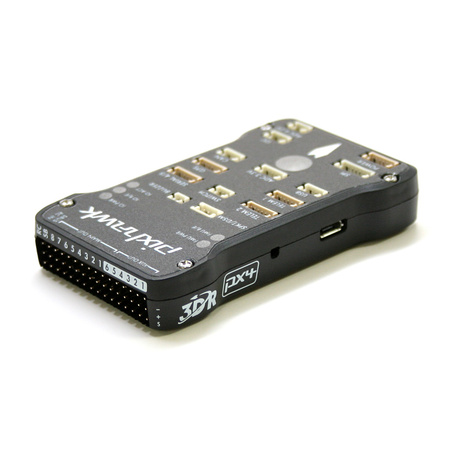
\includegraphics[height = 6cm]{Images/System/Pixhawk.jpg}     
				\caption{Pixhawk Flight Controller}
				\label{IM_Pixhawk}
			\end{figure}
			
			It features a 32 bit STM32F427 processor, running at 168MHz with 256Kb of RAM and a 2Mb Flash. It comes equipped with a full inertial measurement unit (IMU), consisting of a gyroscope, accelerometer and magnetometer. There is also an integrated barometer to adjust flight patterns as the air pressure fluctuates. It has an additional 32 bit co-processor that acts as a failsafe. It has multiple interfacing capabilities as well as a built in power protection unit\footnote{https://pixhawk.org/modules/pixhawk}. 
			
			The Pixhawk has been designed for robotic applications thus is light weight and power efficient. It operates on a real time operating system called \textit{NuttX} which has Unix characteristics but is much lighter than a different operating system such as Linux. This provides a lot of reconfigurability which is wanted in this project.


		\section{Electronic Speed Controller}
		The flight controller will take in information from the onboard sensors. It then sends a motor control command based on that information to the electronic speed controller (ESC), which directly controls the speed of each motor. This subsystem needs to be chosen based on the maximum amount of current it can handle. At 100\% throttle the current draw of the motor should not exceed 75\% of the ESC's limit. Another important consideration is the ESC's refresh rate and computing speed. The flight controller will be rapidly sending data to the ESC. The quicker the module can respond, the more accurately the platform will fly. 
		
		Each ESC has built in intelligence and will have their own dedicated firmware. Most ESCs will come with built in firmware, the design must be tailored for a quadcopter configuration. If not most common ESCs can be reflashed with downloadable open-source software\footnote{http://www.rcgroups.com/forums/showthread.php?t=1513678}.
		
			\subsection{Drone 3's ESC}
		
		\section{On Board Computer}
		Where the flight controller ensures the craft maintains steady flight, the On Board Computer (OBC) handles all higher level processing. This will include interfacing to the on board sensors, the sensor pack as well as handling most of the networking. In an aerial application weight and power consumption are both important considerations. The OBC will have to process streams of data at fast rates to successfully navigate the drone. Based on current available commercial products a few were selected. The advantages and disadvantages of each will are described below.
			
			\subsection{Raspberry Pi 3 Model B}
			
			The Raspberry Pi has become a well known and respected piece of hardware. It has generated a large community and thus resources are readily available and the device can be bought locally. The new version of the device runs a 1.2GHz 64-bit quad-core ARMv8 CPU and includes built in Bluetooth and WiFi modules, an image from the Raspberyy Pi website is shown in Figure \ref{IM_Pi}\footnote{https://www.raspberrypi.org/products/raspberry-pi-3-model-b/}. 
			
			\begin{figure}[H]
				\centering
				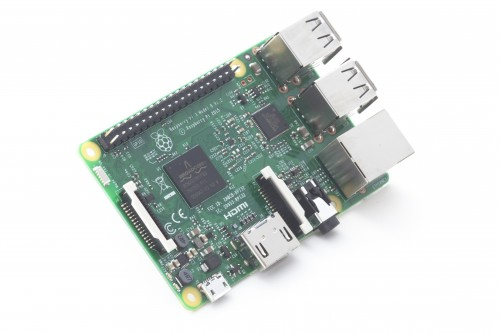
\includegraphics[height = 6cm]{Images/System/Pi.jpg}     
				\caption{Raspberry Pi 3 Model B}
				\label{IM_Pi}
			\end{figure}
						
			It has a large 40 pin GPIO connector, 4 USB connections and an Ethernet port. The Pi's main advantage would be the access to the online community constantly updating Raspberry Pi wikis and forums. With the community also comes example projects and large variety of compatible hardware and open source software. With a maximum current of 2.5A at 5V, the 12.5W computer is relatively low powered which suits this application. However there are more powerful machines that can run more intense algorithms at the cost of more power.
			
			\subsection{Odroid XU4}
			A Korean company, Hardkernel has designed a compact high processing power unit called the Odroid XU4. It has gained respect in some developer communities due to it's incredible processing power. It can run both Android, Ubuntu and other similar Linux based operating systems. Hardkernel has generated an immense of documentation and wiki pages, all available on their website\footnote{http://www.hardkernel.com/}. They also have a team of developers creating new devices to interface with the devices. 
			
			\begin{figure}[H]
				\centering
				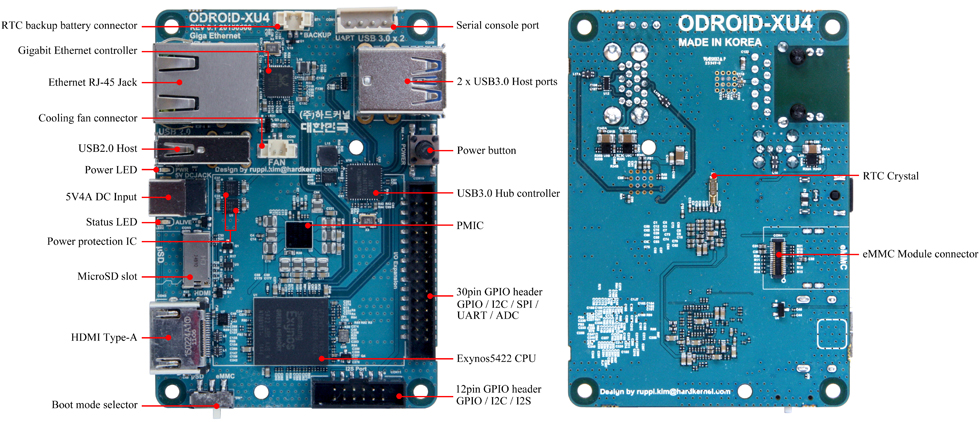
\includegraphics[height = 6cm]{Images/System/XU4.jpg}     
				\caption{The Odroid XU4}
				\label{IM_Odroid}
			\end{figure}
			
			The XU4 hosts a formidable Samsung Exynos5422 Cortex™-A15 processor running at a 2GHz clock speed and an additional Cortex™-A7 Octa core processing unit. This allows for incredible processing capabilities and speed, an image from Hardkernel's Website is shown in Figure \ref{IM_Odroid}. The rated power supply for the unit is a 4A at 5V module. Including a 20W module on board will add a significant drain on the power source. It comes with 2 stable USB 3.0 ports and an additional USB 2.0 connection. 
			
			The Odroid is also frequently used at the CSIR, opening up experience and knowledge on the devices.
			
		\section{Networking}
		A robot that is required to navigate areas where humans cannot access requires a wireless networking solution to send and receive data. This data could be control commands, flight and diagnostic data or sensing information. A reliable connection is an important factor to ensure a successful mission and will be validated against it's speed, packet loss and ultimately reliability.
		
		Generally applications that require far distance use radio frequencies as their means of communication. There are other options, some of which are explored and compared in a design of an intelligent street light \cite{StreetLight}. Here Leccese looks at Bluetooth, WiFi and compares them to a ZigBee module, although the application is different the review of the wireless networking can be useful. 
		
		The ZigBee module is a more useful platform when creating a network containing many devices that all need to interconnect. It has incredible low power abilities and could be looked at further down the line for creating a wireless mesh network in an underground mine to better communications. Bluetooth has limited range and doesn't produce adequate performance for this application. WiFi could also be a good communication system and can be looked at for point to point communication to the OBC. WiFi has decent range with high transmission speeds creating a more power hungry system compared to the ZigBee modules and other RF devices.
		
		The design may also look at including multiple communication peripherals as a fail-safe in case communications is lost to the base station. The base station will be the control point for the craft. The pilot needs full control through it and any relevant data that needs to be transmitted will be sent here as well.
		
		

		
		\section{Location}
		An important part of any robotic application is localisation. As stated earlier, an underground environment limits the use of traditional GPS. Stellenbosch University as well as the CSIR are both funding research into localisation in a GPS constraint environment \todo{Would be great to cite Natasha or ESL here}. Until such a time that these technologies are readily available, this project will work with traditional GPS devices.
			
		As discussed previously, this project will not be designing for a GPS constraint environment. Fortunately there are many commercial  GPS modules available for purchase. Each with their own advantages and disadvantages. For this project the module needs to be lightweight and low power. The GPS needs to create speed and translation data, this information is crucial when generating maps of unknown areas. The PixHawk website recommends the 3DR uBlox GPS kit\footnote{https://store.3dr.com/products/3dr-gps-ublox-with-compass}. Although many alternatives exist, the open source hardware status creates ease of integration and support. With these considerations, this module has been chosen.
			
		It weighs a total of 16.8gs and as has a low 8.5mm profile. With an update rate of 5Hz and built in compass. This module will perform adequately and fulfil the design needs of the project.
			 
		\section{Object Avoidance}
		Due to the mature of the project object avoidance is deemed an important attribute to design for. This requires that the drone has an understanding of it's environment. This information can then be used in higher processing nodes to actively avoid objects. A few different sensor variations are observed below. 
	
			\subsection{Time of Flight}		
			The first and most common would be using a time of flight (TOF) sensor, such as an ultrasonic transducer. Very similar to bats, a sonar module will emit a pulse and based on the time it takes for the signal to return the distance can accurately be measured. A sonar is dependant on a lot of variables and would require calibration for the environment it is in. Due to the method the modules acquire information the drone will be receive a speed limitation, this fortunately agrees with the desired steady flight dynamics. Since the sonar is dependant on the density of the medium it travels through, disturbance created by the rotors could severely affect the performance of the sensors.
			
			Another option in the same category would be to use an infra red (IR) transceiver in the same configuration. The system uses strobed IR pulses to monitor the distance of an object, the system depends on the ratio of reflection for the IR spectrum. If an object as a high refraction ir absorption ratio the signal can get lost. Ambient light can also cause interference, although most modules will have built in filters.
			
			Using the same base technology TOF cameras have been developed such as Microsoft's Kinect. Instead of a single point, a TOF camera projects an IR grid into the area it wishes to explore. By measuring deviations in the expected grid structure, distance information can be inferred. In an IR rich environment, TOF cameras can get overwhelmed and produce unreliable results. Due to the projection, the power requirements of such a system can also be high.
			
			\subsection{Image Processing}
			The term image processing has been used here to discuss a system that can extract data through a camera feed. It is well known that stereo vision can produce 3D information from multiple 2D images. Although more processing is required, very good results can be obtained form this set up. Generally these systems can be slow and clunky with a high power draw and weight due to the multiple required modules. Using multiple camera streams can also be a relatively slow process, thus limiting the speed of the craft severely.
		
			However, reliability from a robust image processing unit will be more reliable and consistent than a different system. Barry in his PhD developed such a design that minimises the discussed negative effects \cite{Barry2016}. Using this design MIT could obtain object avoidance at speeds of 31mph, proving the effectiveness of the object avoidance system.
			
			Regardless of the modules chosen, object detection and avoidance will be looked at in more detail further into the project.
			
		\section{Lighting}
		Since the drone is required to conduct surveys of unknown areas, the possibility exists where the platform is required to illuminate the area it needs to monitor. This requirement hints at the need for an embedded lighting system. Bright lights can be a power hungry system even if designed correctly. The exact specifications will be discussed further in the text but does not form part of project scope.
		
		LEDs will be used for their performance, longevity and power saving characteristics. They will require an LED driver with dimming capabilities to limit the power usage when full brightness is not needed. The illumination will be able to help the sensor pack gather credible surveying data
		
		
		\section{Sensor Pack}
		The actual sensor pack in question is remaining generic. So that the platform can cater for an array of sensing devices and applications. To ensure compatibility, the sensor pack needs to be able to powered as well as communicated to. It will have access to interface directly to the OBC.
		
		The actual sensing element could vary between 
		\todo[inline]{Lidar}

		\section{Power Supply}
			\subsection{Electrical Requirements Analysis}
			\subsection{Power Source}
			\subsection{Power Management}
			\todo{Power Monitoring}
			\todo{Charging Scheme}


